\chapter{Tinjauan Pustaka}

Pada bab ini berisi hasil tinjauan pustaka yang menjadi dasar analisis dan perancangan pada BAB III. Bab ini secara garis besar berupa teori keamanan perbatasan jaringan, tinjauan pustaka mengenai permasalahan yang dihadapi, solusi teoritis, dan tinjauan pustaka yang berkaitan dengan perancangan solusi. Solusi teoritis berupa klasifikasi deteksi intrusi, yakni \textit{anomaly-based} dan \textit{signature-based}.

\section{\textit{Network Border Security}}

Seperti dalam dunia nyata, sebuah keamanan dijaga pada sebuah wilayah tertentu. Pada sebuah jaringan border-security memisahkan jaringan \textit{internal} dan \textit{external}. Jaringan \textit{internal} sebagai yang akan dilindungi, dan memisahkannya dengan external network menggunakan sebuah gateway border. Pada (Strebe, 2004) border-security secara teori harus memiliki \textit{measures} sebagai berikut:

\begin{enumerate}
	\item \textit{Control every crossing}
	
	Border security harus melakukan pengecekan untuk setiap lalu lintas data antara internal network dan external network. Sebuah koneksi antara internal network dan external network yang tidak dilakukan pengecekan
	dapat menjadi celah untuk terjadinya serangan. Hal ini dapat dilakukan dengan cara menempatkan firewall pada setiap batas jaringan.
	
	\item \textit{Apply the same policy universally}
	
	Sebuah control untuk sebuah lalu lintas data tertentu harus dilakukan sama untuk seluruh hubungan yang terjadi antara internal network dan external network. Hal ini membutuhkan penerapan menyeluruh, karena efek dari penerapan ini akan bergantung pada penerapan yang terlemah. Jika dibutuhkan perbedaan tingkat keamanan, bisa dilakukan dengan memisahkan jaringan yang memerlukan perbedaan tingkat. Salah satunya seperti yang dilakukan pada DMZ.
	
	\item \textit{Deny by default}
	
	Seluruh keterhubungan hanya akan memperbolehkan lalu lintas data yang ada pada whitelist. Penerapan ini perlu dilakukan untuk lalu lintas ke luar	maupun ke dalam firewall. Jika sebaliknya diterapkan \textit{allow by default}, ketika malware dengan jenis trojan tanpa sengaja dijalankan pada jaringan internal, malware dapat dengan mudah melakukan koneksi ke luar. Misal untuk mengirimkan data yang seharusnya dilindungi.
	
	\item \textit{Hide as much as information as possible}
	
	Penyembunyian data interior dari sebuah network perlu dilakukan. Hal ini digunakan untuk mencegah penyerang mendapatan informasi jaringan internal. Mendapatkan informasi mengenai jaringan internal merupakan langkah awal yang dilakukan \textit{hacker}. Jika informasi ini didapatkan, hacker dapat menggunakan untuk berbagai macam, seperti \textit{inserting-traffic at IDS} (\cite{marpaung2012survey}).
	
\end{enumerate}

\section{Firewall}
Firewall merupakan hardware, software atau kombinasi keduanya yang digunakan untuk melakukan monitoring dan filter terhadap lalu lintas data yang masuk atau keluar dari sebuah jaringan yang berusaha dilindungi (Kizza, 2005). Menurut (Stallings, 2012) \textit{design goal firewall} sebagai berikut: 
Seluruh lalu lintas data dari dalam ke luar ataupun sebaliknya harus melalui firewall;
Hanya lalu lintas data yang terotorisasi yang dapat melalui firewall;
dan firewall merupakan system yang kebal terhaadap penetration.

Kekuatan dan kelemahan dari firewall menurut (Peterson, 2012):
Firewall dapat dideploy unilaterally;
Firewall tidak dapat membatasi akses antara host yang berada dalam internal-network;
Jika pihak diberikan akses ke internal-network, maka pihak tersebut menjadi security vulnerability;
Dan bug pada firewall yang dapat diakses dari internal-network dapat menjadi masalah serius.

Firewall saat ini yang pada umumnya memiliki tipe sebagai berikut:

\begin{enumerate}
	\item \textit{Packet filtering firewall}
	\textit{Packet filtering firewall}
	
	Merupakan firewall yang menggunakan informasi dari protokol IP untuk menentukan apakah dilakukan teruskan atau buang untuk lalu lintas data masuk maupun keluar.
	
	\item \textit{Application proxy firewall}
	
	Application proxy firewall atau application gateway merupakan firewall yang digunakan pada application layer untuk sebuah protocol tertentu.
\end{enumerate}

\subsection{Arsitektur Firewall}
Firewall pada implementasinya dapat ditempatkan dengan beberapa arsitektur menurut (\cite{zwicky2000building}).

\subsubsection{Arsitektur \textit{Dual-Homed Host}}

Arsitektur \textit{dual-homed host} merupakan dibangun dengan menggunakan komputer \textit{dual-homed host}, yakni sebuah komputer yang terhubung dengan dua atau lebih jaringan. Komputer ini dapat bekerja sebagai router antara kedua jaringan yang terhubung ke komputer tersebut. Namun, untuk mengimplemntasi firewall dengan arsitektur \textit{dual-homed host} fungsi routing ini tidak difungsikan. Sehingga tidak ada data yang dapat dikirimkan langsung antar kedua jaringan. Jadi untuk setiap paket yang akan dikirimkan dari jaringan internal ke jaringan luar harus melalui \textit{dual-homed host}, dan dari jaringan luar ke jaringan dalam juga harus melalui \textit{dual-homed host}. Sehingga susunan komponen pada jaringan tersebut seperti pada gambar \ref{fig:dual_homed}

\begin{figure}[H]
	\centering
	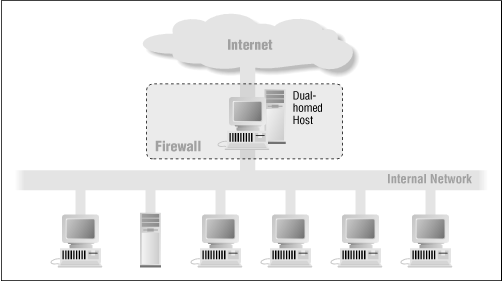
\includegraphics[width=300px]{resources/dual_homed.png}
	\caption{Arsitektur \textit{Dual-Homed}}
	\label{fig:dual_homed}
\end{figure}

\subsubsection{Arsitektur \textit{Screened Host}}

Berbeda dengan arsitektur \textit{dual-homed host} yang memberikan service dari host yang terhubung ke beberapa jaringan dengan fungsi tidak mengaktifkan fungsi routing, arsitektur \textit{screened host} memberikan layanan dari host yang hanya terhubung ke internal network dan menggunakan router terpisah seperti pada  gambar \ref{fig:screened_host}. Pada arsitektur ini, keamanan dijaga oleh packet filtering, dengan melakukan konfigurasi berikut:

\begin{enumerate}
\item Memperbolehkan \textit{internal host} untuk dapat mengakses beberapa service langsung tanpa melalui proxy.
\item Melarang semua paket dari internal host. (Untuk memaksa host itu menggunakan proxy).
\end{enumerate}

Namun pada pada arsitektur ini, jaringan internal sangat mudah diserang dari host \textit{bastion} yang berada pada internal network. Sehingga bastion host menjadi sasaran yang paling diinginkan oleh penyerang. Karena tidak ada pertahanan lagi diantara internal host dan host lain yang berada pada jaringan internal.

\begin{figure}[H]
	\centering
	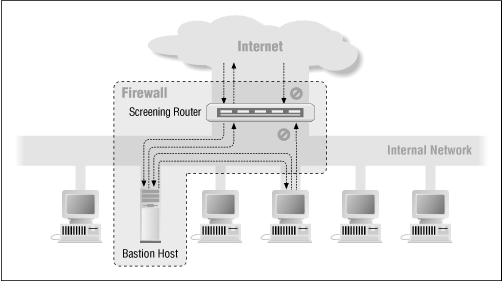
\includegraphics[width=300px]{resources/screened_host.png}
	\caption{Arsitektur \textit{Screened Host}}
	\label{fig:screened_host}
\end{figure}

\subsubsection{Arsitektur \textit{Screened Subnet}}

Arsitektur \textit{screened subnet} memiliki layer tambahan dibandingkan dengan arsitektur \textit{screened host} dengan memisahkan internal network lebih jauh dari Internet.

Arsitektur ini ditujukan agar host \textit{bastion}, yakni host yang dieskpos ke Internet, merupakan host yang paling rentan untuk diserang. Meskipun host sudah dilakukan usaha untuk melindungi host tersebut, namun host tersebut menjadi titik paling jelas untuk diserang.

\begin{figure}[H]
	\centering
	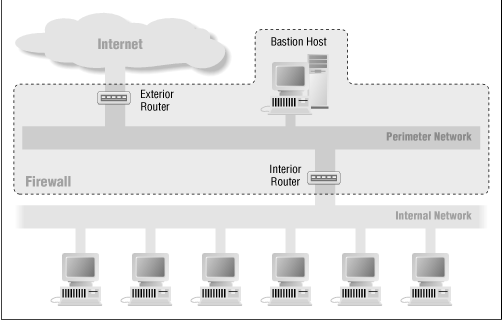
\includegraphics[width=300px]{resources/screened_subnet.png}
	\caption{Arsitektur \textit{Screened Subnet}}
	\label{fig:screened_subnet}
\end{figure}

\section{Next Generation Firewall}
Pada masa ini, firewall terbagi menjadi 2 yaitu tradisional firewall dan new generation firewall. Hal ini terjadi karena tradisional firewall tidak lagi mumpuni untuk menahan serangan yang ada di dunia internet ini. 
Tradisional firewall adalah firewall yang bekerja di \textit{network layer}(\cite{nicoll2004challenges}), menggunakan port dan protokol IP untuk mengontrol dan mencegah serangan dari jaringan.(\cite{zhong2012design}) Skema dari tradisional firewall ini dapat dilihat pada gambar berikut.
\begin{figure}[H]
	\centering
	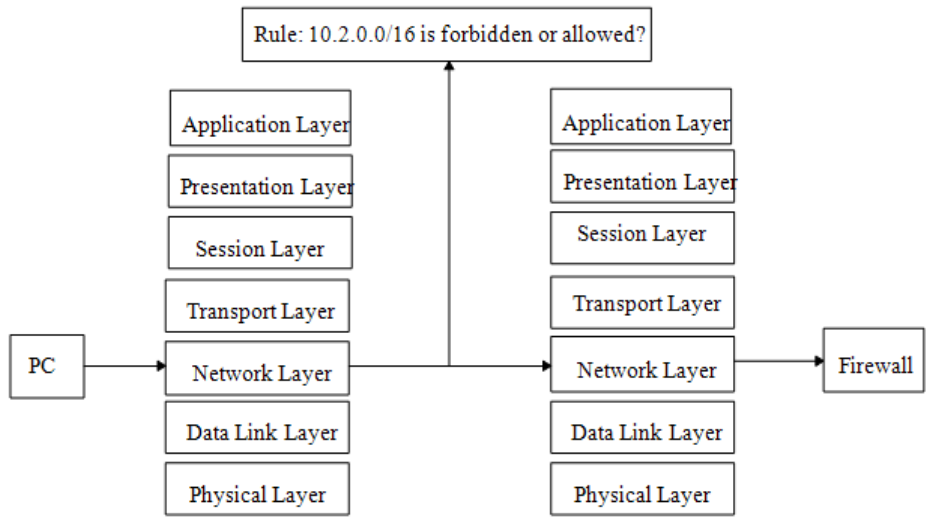
\includegraphics[width=0.8\textwidth]{resources/tradisional_firewall.png}
	\caption{Skema tradisional firewall(\cite{zhong2012design})}
	\label{fig:tradisional_firewall}
\end{figure}

Firewall ini hanya mengecek header paket sesuai dengan portnya, sehingga tidak dapat mengontrol aplikasi. Tradisional firewall yang memakai \textit{deep packet inspection} (DPI) untuk menambah keamanan juga tidak terlalu berhasil, karena memunculkan limitasi dan masalah baru. Menurut (\cite{miller2011next}), masalah tersebut adalah
\begin{itemize}
	\item Aplikasi yang tidak seharusnya berada di jaringan diperbolehkan masuk ke jaringan.
	\item Tidak semua paket yang harus diperiksa terperiksa
	\item Policy management menjadi rumit dan berbelit
	\item Performansi yang tidak memadai 
\end{itemize}

Sementara itu, Next Generation Firewall (NGFW) merupakan pengembangan dari first-generation firewall yang memiliki Deep Packet Inspection (DPI). Secara fungsionalitas NGFW merupakan gabungan dari IPS dan first-generation firewall. NGFW dapat dipandang sebagai IPS karena NGFW memiliki awareness terhadap application level payload. Hasil pengecekan kemudian digunakan untuk memutuskan apakah paket di-forward atau di-drop. (Pescatore, 2009). New Generation Firewall adalah firewall yang berjalan diatas layer aplikasi, untuk mendeteksi apakah paket tersebut sesuai dengan user`s rule atau tidak(\cite{zhong2012design}). Skema dari new generation firewall adalah sebagai berikut.
\begin{figure}[H]
	\centering
	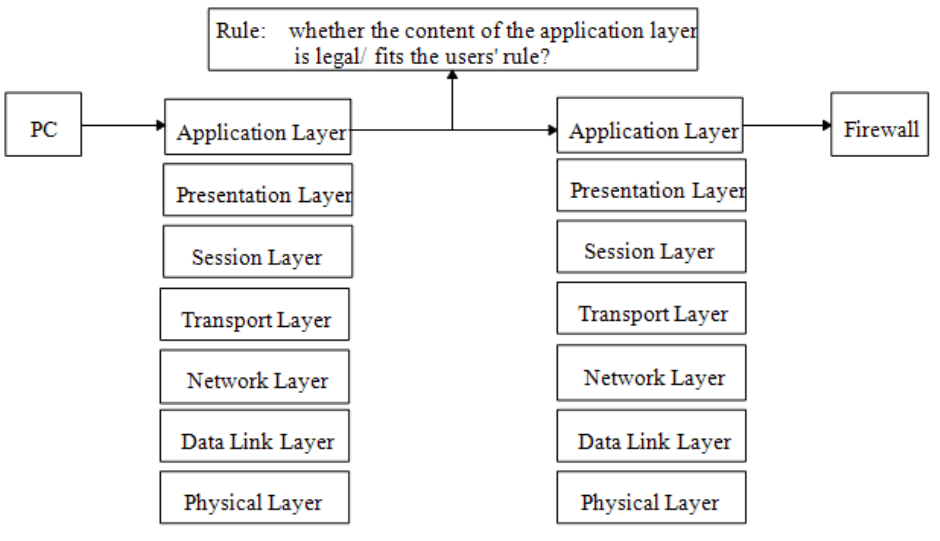
\includegraphics[width=\textwidth]{resources/NGFW.png}
	\caption{Skema new generation firewall(\cite{zhong2012design})}
	\label{fig:new_generation_firewall}
\end{figure}

Fungsi dan kemampuan utama yang dibutuhkan oleh new generation firewall adalah:
\begin{itemize}
	\item Identifikasi aplikasi (port, protocol, evasive techniques, atau SSL encryption) sebelum melakukan hal apapun
	\item Menyediakan policy-based control yang lebih jelas dan granular
	\item Secara akurat mengidentifikasi pengguna dan menggunakan informasi tersebut sebagai atribut dari policy control
	\item Menyediakan proteksi secara real-time terhadap ancaman dari jaringan, termasuk yang beroperasi pada layer aplikasi.
	\item Terintegrasi untuk meningkatkan kapasitas pencegahan ancaman
\end{itemize}

\subsection{Teknik Identifikasi aplikasi}
Teknik Identifikasi aplikasi yang digunakan oleh new generation firewall adalah
\begin{itemize}
	\item Deteksi dan dekripsi aplikasi protokol\\
	Untuk mendeteksi protokol aplikasi sehingga dapat dianalisis lebih lanjut
	\item Decode aplikasi protokol\\
	Untuk mendeteksi apakah ada aplikasi lain yang berjalan melalui protokol tersebut (tunnel), seperti Yahoo! Instant Messenger yang mungkin berada di dalam protokol HTTP
	\item Application signatures\\
	Untuk mengecek apakah aplikasi tersebut menggunakan port dan protokol yang sesuai dengan fungsinya.
	\item Heuristics
\end{itemize}

\subsection{User identification}
Teknologi ini mengidentifikasi user sehingga dapat digunakan untuk:
\begin{itemize}
	\item Mendapatkan visibilitas tentang siapa yang bertanggung jawab untuk semua aplikasi, konten, dan ancaman lalu lintas data pada jaringan tersebut
	\item Mengizinkan penggunaan identitas sebagai variabel dalam access control policies.
	\item Memfasilitasi troubleshooting/incident response
\end{itemize}

\subsection{Content identification}
Teknologi ini membuat next generation firewall dapat mencegah ancaman secara real-time, mengontrol web surfing activities, dan memfilter file atau data. Komponen dari teknologi ini adalah:
\begin{itemize}
	\item Pencegahan ancaman\\
	Komponen ini berfungsi untuk mencegah spyware, virus, dan ancaman lainnya dari jaringan. Komponen ini dibantu oleh application decoder, stream-based virus detection, spyware scanning, uniform threat signature format, dan IPS.
	\item URL filtering\\
	Komponen ini memfilter konten melalui URL.
	\item Filter file dan data\\
	Komponen ini menggunakan kelebihan dari in-depth application inspection untuk mengurangi pengiriman file dan data yang tidak terotorisasi. 
\end{itemize}

\subsection{Perbedaan performansi antara tradisional firewall dan new generation firewall}
Pada tradisional firewall, fungsi-fungsi keamanan dilakukan secara terpisah satu sama lain, seperti yang digambarkan pada gambar \ref{fig:architecture_tradisional_firewall}. Hal ini menyebabkan penggunaan system resource yang berlebihan dan tidak efisien.
\begin{figure}[H]
	\centering
	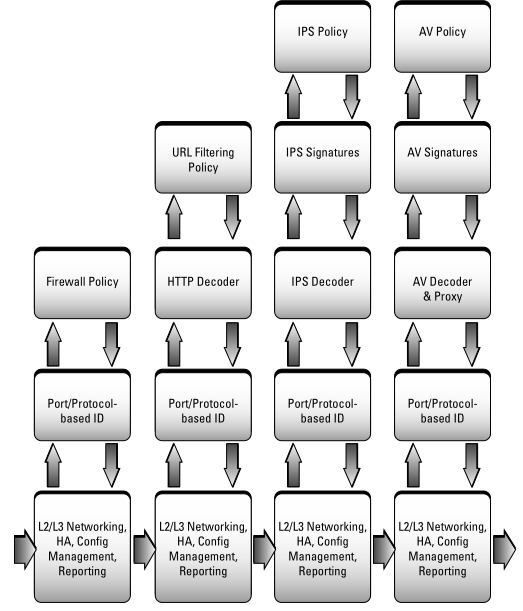
\includegraphics[width=8cm]{resources/architecture_tradisional_firewall.png}
	\caption{arsitektur proses tradisional firewall(\cite{miller2011next})}
	\label{fig:architecture_tradisional_firewall}
\end{figure}

Sebaliknya, new generation firewall menggunakan single-pass architecture untuk mengeliminasi pengecekan paket secara repetitif, mengurangi beban pada hardware dan meminimalkan latency, seperti yang dapat dilihat pada gambar berikut.

\begin{figure}[H]
	\centering
	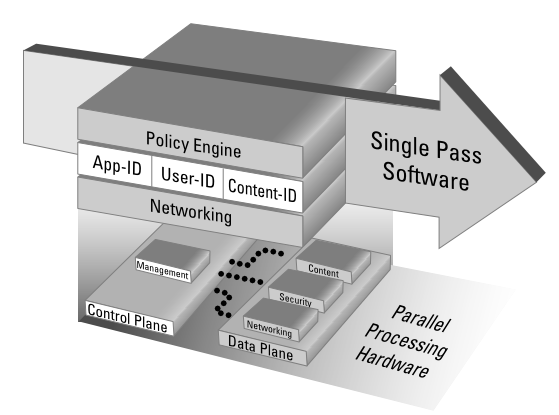
\includegraphics[width=0.7\textwidth]{resources/architecture_NGFW.png}
	\caption{arsitektur proses new generation firewall(\cite{miller2011next})}
	\label{fig:architecture_NGFW}
\end{figure}

\section{Deep Packet Inspection}
Deep Packet Inspection (DPI) adalah salah satu teknologi utama untuk mengidentifikasi dan mengotentikasi protokol dan aplikasi yang dibawa bersama IP(\cite{allot2007digging}). \textit{Standard packet inspection process} hanya mengekstrak informasi dasar dari suatu protokol seperti IP address (tujuan, sumber) dan informasi koneksi low-level lainnya, yang biasanya berada pada header paket tersebut. Inspeksi ini tidak mendapatkan informasi yang cukup untuk dapat menyimpulkan apakah aplikasi tersebut aman atau tidak. 
\begin{figure}[H]
	\centering
	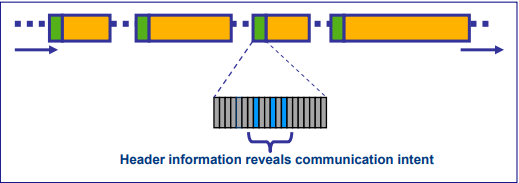
\includegraphics[width=0.8\textwidth]{resources/standard_inspection.png}
	\caption{standard packet inspection (\cite{allot2007digging})}
	\label{fig:standard_inspection}
\end{figure}
Sebaliknya, DPI menyediakan informasi tentang aplikasi tersebut. Hal ini dicapai dengan menganalisis konten pada header paket dan payload paket pada suatu transaksi paket. Oleh karena itu, DPI dapat menyediakan kemampuan untuk menganalisa penggunaan jaringan dan mengoptimasi performansi jaringan. 

Komponen yang digunakan untuk memberi identitas pada aplikasi dan protokol disebut signature. Signature ini dapat juga diumpamakan seperti fingerprint pada manusia, dimana tidak ada yang sama satu dengan yang lainnya. Oleh karena itu, signature digunakan untuk mengidentifikasi aplikasi dan protokol. Signature pada aplikasi harus dicek secara berkala, karena signature tersebut dapat berubah seiring aplikasi update atau revisi protokol.

Walaupun signature tersebut dikembangkan dengan tujuan keunikan dan untuk mengidentifikasi suatu aplikasi atau protokol, ada kalanya signature tersebut tidak robust. Terdapat istilah \textit{false positives} dan \textit{false negatives} karena signature tersebut. \textit{False positives} merujuk pada keadaan salah mengelompokkan atau salah mengidentifikasi, seperti suatu aplikasi diidentifikasi sebagai sesuatu, namun sebenarnya bukan. \textit{False negatives} merujuk pada keadaan dimana suatu aplikasi atau protokol tidak teridentifikasi secara konsisten sebagai sesuatu yang sama. Contohnya, beberapa aplikasi akan berperilaku berbeda apabila koneksi yang dilakukan melalui proxy atau tidak. Salah satu cara untuk membuat signature tersebut menjadi lebih robust adalah dengan menggunakan beberapa pola kombinasi.

\subsection{Metode analisis signature}
Ada beberapa metode analisis yang digunakan untuk mengidentifikasi dan mengelompokkan paket, yaitu:
\begin{itemize}
	\item Analisis berdasarkan port\\
	Analisis ini merupakan analisis yang paling mudah dan paling dikenal. Namun analisis ini tidak cukup untuk mengidentifikasi aplikasi sendirian, dikarenakan sudah banyak aplikasi yang memakai random port atau menyamar sebagai aplikasi lain pada port tertentu.
	\item Analisis berdasarkan string match\\
	Analisis ini akan mencari suatu string pada konten paket tersebut. Hal ini dilakukan karena banyak aplikasi yang menyertakan nama aplikasi tersebut pada protokolnya. 
	\item Analisis berdasarkan numerical properties\\
	Analisis ini melibatkan perhitungan dan karakteristik numerik pada paket tersebut, seperti payload length, banyaknya paket yang dikirim untuk respon transaksi tertentu, dan numerical offset dari suatu string dalam paket tersebut. Analisis ini juga tidak cukup berdiri sendiri untuk mengidentifikasi aplikasi.
	\item Analisis berdasarkan perilaku dan heuristics\\
	Analisis ini merujuk pada bagaimana biasanya protokol berperilaku dan beroperasi. Analisis heuristik pada umumnya berasal dari hasil statistik dari paket yang diamati.
\end{itemize}

\section{Malware}
\textit{Malicious software} menurut (\cite{idika2007survey}) memiliki banyak baentuk salah satunya adalah Malicious Code (MC). Menurut (\cite{attackingmalcode}), malicious code merupakan kode yang ditambahkan, diubah, atau dihilangkan dari sistem software untuk membahayakan atau mengubah fungsi yang diharapkan dapat dilakukan oleh sistem.

Virus merupakan program komputer yang mereplikasi dengan menyisipkan dirinya ke program lain. Program yang disisipi oleh virus menjadi terinfeksi disebut inang. Hal ini yang membedakan virus dengan malware lain, untuk melakukan fungsinya virus memerlukan inang (\cite{attackingmalcode}).

Worm merupakan program komputer yang mereplikasi dirinya dengan menjalankan kode worm yang manjadi sebuah program tersendiri. Bagian yang membedakan worm dan virus, worm tidak memerlukan inang untuk melakukan fungsinya. Selain itu, virus dan worm juga berbeda pada cara penyebarannya. Pada umumnya, virus berusaha untuk menyebar melalui file atau program pada satu komputer. Sedangkan worm berusaha untuk menginfeksi sebanyak mungkin komputer melalui jaringan (\cite{attackingmalcode}).

Trojan horse merupakan malicious code yang tambahkan oleh desainer dalam sebuah aplikasi atau sistem. Aplikasi tersebut menjalankan fungsinya, namun melakukan aktifitas malicious seperti merekam kegiatan pengguna dan mengirimkannya ke pembuatnya. Trojan horse pada umumnya berkaitan dengan mengakses dan mengirimkan informasi tanpa otorisasi dari pengguna. Trojan horse dapat dikategorikan sebagai spyware. 


\section{Malware Detection}

Pada (\cite{idika2007survey}) teknik untuk mendeteksi malware dibedakan menjadi dua, yakni: signature-
based dan anomaly-based. Terdapat bentuk khusus anomaly-based yakni specification-based. Setiap teknik memiliki jenis static, dynamic, dan hybrid.

\subsection{Anomaly-based Detection}

Pada (\cite{idika2007survey}) dijelaskan, anomaly-based detection memiliki dua fasa, yakni fasa training, dan fasa deteksi. Pendeteksian jenis ini memiliki kelebihan, yakni dapat mendeteksi serangan yang sebelumnya belum dikenali. Namun, deteksi jenis ini memiliki tingkat kesalahan pendeteksian yang tinggi. Anomaly based-detection melakukan pendeteksian dengan cara membuat pendekatan perilaku yang valid dilakukan oleh sebuah sistem.

\begin{figure}[H]
	\centering
	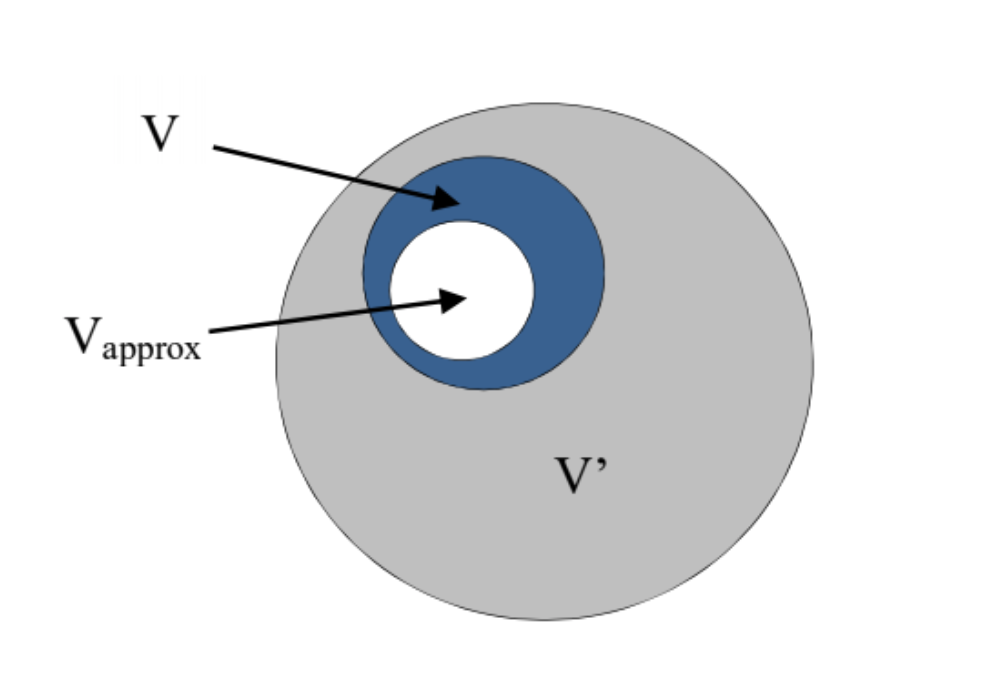
\includegraphics[width=220px]{resources/anomaly_illustration.png}
	\caption{Ilustrasi karakterisasi perilaku pada anomaly-based detection}
	\label{fig:anomaly_illust}
\end{figure}

Gambar \ref{fig:anomaly_illust} menggambarkan bagaimana anomaly-based detection mengkarakterisasi perilaku sistem. V merupakan himpunan perilaku yang tidak bertentangan dengan requirement. V’ merupakan himpunan perilaku yang yang tidak valid. Vapprox merupakan hasil pendekatan yang dilakukan oleh anomaly-based detection.

\subsection{Signature-based Detection}
Signature-based detection dalam (\cite{idika2007survey}) merupakan teknik yang menggunakan malicious-model untuk mendeteksi malware. Kumpulan dari malicious-model (signature) menjadi knowledge base dari system pendeteksi jenis ini. Sehingga pada Gambar \ref{fig:signature_illust}, diilustrasikan bahwa S (kumpulan signature) merupakan subset dari U yang merupakan seluruh signature dari perilaku malicious. Karena keterbatasan media penyimpanan, S akan sangat kecil jika dibandingkan dengan U yang sangat besar.

\begin{figure}[H]
	\centering
	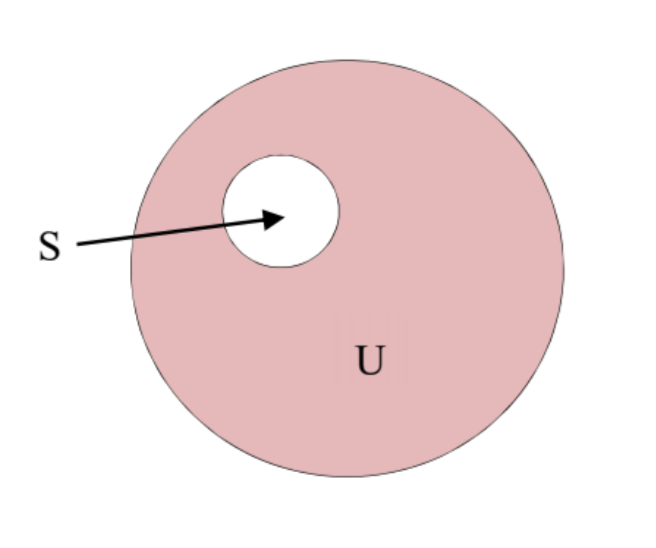
\includegraphics[width=190px]{resources/signature_illustration.png}
	\caption{Ilustrasi himpunan signature terhadap seluruh malicious signature}
	\label{fig:signature_illust}
\end{figure}

\section{Iptables}
Pada(\cite{rash2007linux}) dijelaskan, Iptables firewall dikembangkan oleh NetFilter Project \textit{(http://www.netfilter.org)}, dan sudah menjadi bagian dari kernel linux sejak Januari 2001.  Pada masa ini, Iptables sudah banyak digunakan pada firewall komersial. Hal ini dikarenakan Iptables mempunyai protokol \textit{state tracking} yang komprehensif, \textit{packet application layer inspection}, pembatasan kecepatan, dan mekanisme untuk mengatur \textit{filtering policy} yang mumpuni. 
Istilah Iptables dan Netfilter cukup membingungkan untuk banyak orang pada komunitas Linux. Menurut (\cite{purdy2004linux}) Netfilter adalah bagian dari kernel Linux yang berfungsi untuk memproses paket dari jaringan. Sementara itu,  iptables adalah perintah untuk mengatur \textit{Netfilter} yang dapat digunakan pada \textit{user-space}. 

Suatu iptables policy dibuat dari suatu set aturan yang akan mengatur rute dari suatu paket. Setiap set aturan tersebut diaplikasikan pada chain didalam satu table tersendiri. Table tersebut dikelompokan berdasarkan fungsinya, yaitu filter, \textit{Network address translation} (NAT) dan Packet mangling. Fungsi dari filter adalah untuk mengatur keluar masuknya paket yang masuk ke komputer tersebut. Fungsi NAT digunakan dengan \textit{connection tracking} untuk melakukan Network Address Translation (NAT). Dan yang terakhir, fungsi Packet mangling digunakan untuk menanipulasi paket.

\subsection{Alur pemrosesan paket}
Setiap table memiliki \textit{chain} (urutan) pemrosesannya masing-masing. Alur pemrosesan dasar tersebut dapat dilihat pada gambar-gambar dibawah ini.
\begin{figure}[H]
	\centering
	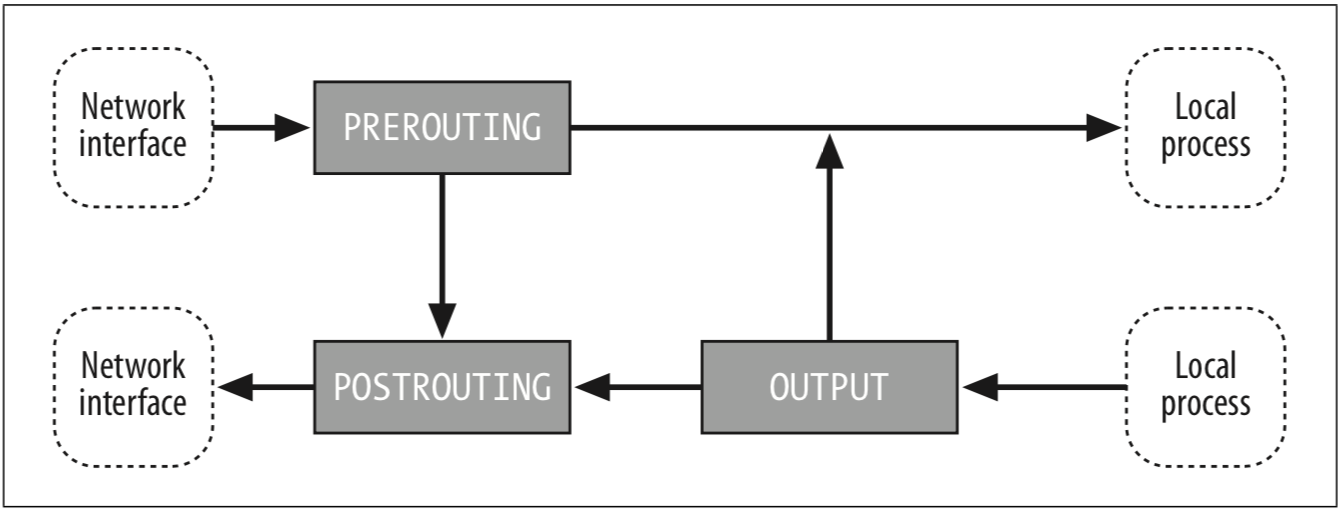
\includegraphics[width=\textwidth]{resources/nat_table.png}
	\caption{Alur pemrosesan paket dan \textit{hook} yang digunakan pada tabel \textit{NAT}. (\cite{purdy2004linux})}
	\label{fig:packetflow_NAT}
\end{figure}

\begin{figure}[H]
	\centering
	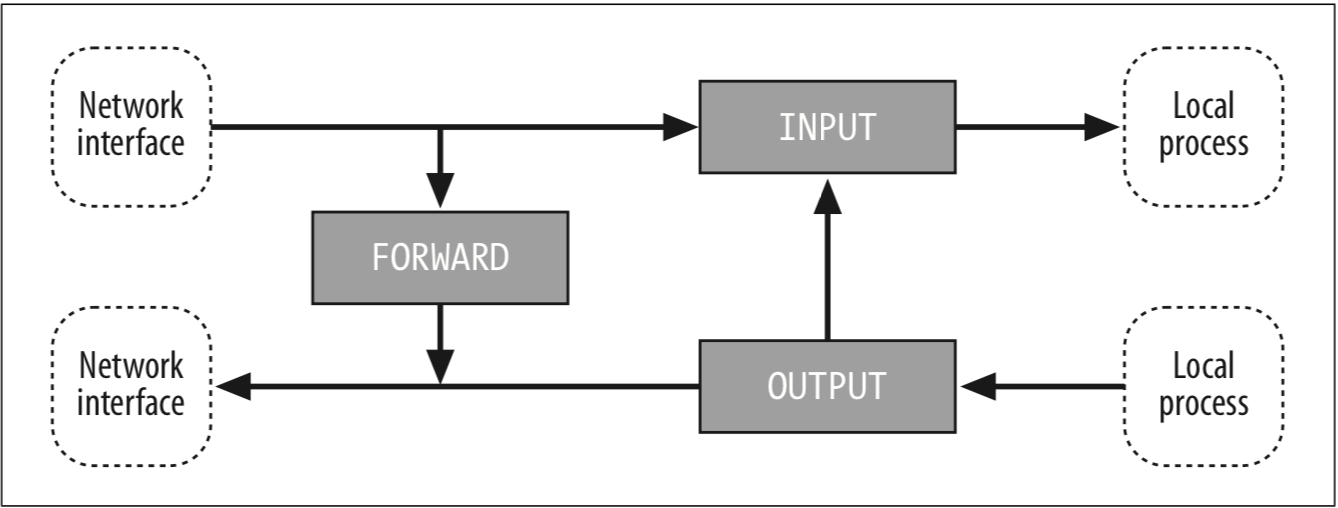
\includegraphics[width=\textwidth]{resources/filter_table.png}
	\caption{Alur pemrosesan paket dan \textit{hook} yang digunakan pada tabel \textit{filter}.(\cite{purdy2004linux})}
	\label{fig:packetflow_filter}
\end{figure}

\begin{figure}[H]
	\centering
	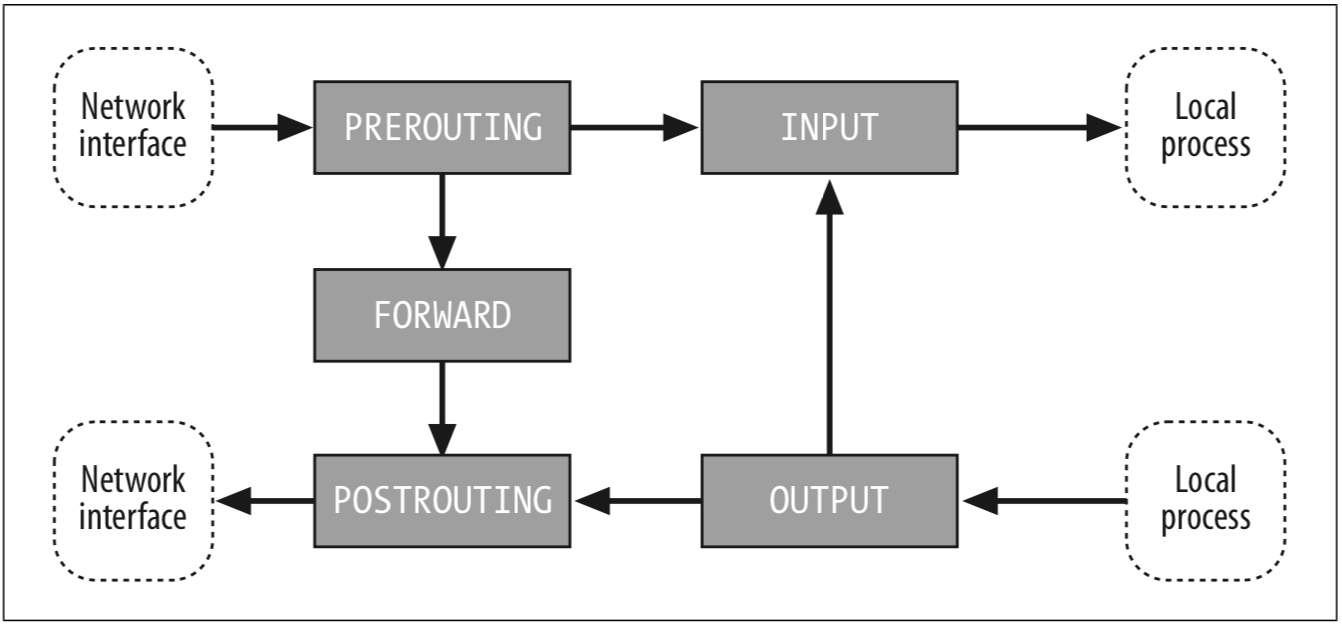
\includegraphics[width=\textwidth]{resources/mangling_table.png}
	\caption{Alur pemrosesan paket dan \textit{hook} yang digunakan pada tabel \textit{mangling}.(\cite{purdy2004linux})}
	\label{fig:packetflow_mangling}
\end{figure}

Poin-poin yang terdapat pada gmabar-gambar diatas adalah hook poin yang memiliki fungsi-fungsi tersendiri.\textit{Netfilter} memiliki 5 poin (\textit{hook}) didalam alur pemrosesan paket, yaitu : \textit{PREROUTING}, \textit{INPUT}, \textit{FORWARD}, \textit{POSTROUTING}, \textit{POSTROUTING}, dan  \textit{OUTPUT}. 
Poin \textit{PREROUTING} akan memproses paket yang baru datang dari \textit{network interface} (setelah melalui proses pengecekan \textit{checksum}).
Poin \textit{INPUT} akan memproses paket yang akan dilanjutkan ke proses lokal.
Poin \textit{FORWARD} akan memproses paket yang keluar masuk melalui \textit{gateway} komputer.
Poin \textit{POSTROUTING} akan memproses paket yang akan meninggalkan \textit{network interface}.
Poin \textit{OUTPUT} akan memproses paket yang baru saja melewati proses lokal.


Built-in chain yang paling umum dipakai untuk membuat firewall adalah INPUT, OUTPUT dan FORWARD, yang berada pada filter table. INPUT chain akan dijalankan satu-persatu oleh paket yang seharusnya memasuki sistem lokal, sementara OUTPUT chain akan dijalankan satu persatu oleh paket yang berasal dari sistem lokal tersebut. Sedangkan FORWARD chain, oleh paket yang melewati sistem tersebut yang bukan ditujukan untuk sistem lokal. Untuk lebih jelasnya, dapat dilihat pada gambar dibawah ini (\ref{fig:iptables_packet_flow}). 
\begin{figure}[H]
	\centering
	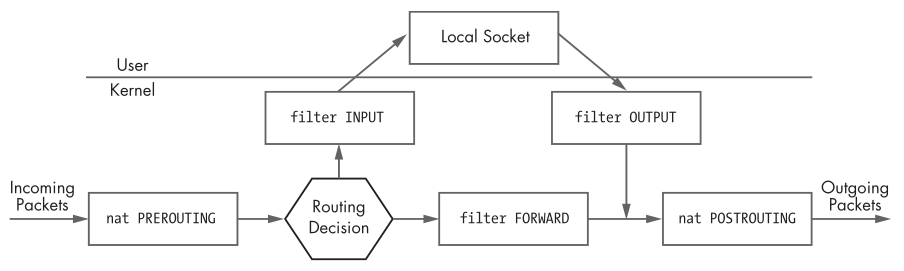
\includegraphics[width=\textwidth]{resources/iptables_packet_flow.png}
	\caption{Contoh alur pemrosesan paket yang melewati tabel NAT dan tabel filter.(\cite{rash2007linux})}
	\label{fig:iptables_packet_flow}
\end{figure}

Paket yang melewati \textit{chain} akan terkena aturan sesuai dengan urutannya. Apabila paket tersebut tidak sesuai kriteria, maka paket akan bergerak ke aturan selanjutnya. Jika paket tersebut tidak memenuhi kriteria sampai aturan yang paling akhir, maka paket tersebut akan diperlakukan sesuai dengan \textit{chain\textquotesingle s policy}. 
Berdasarkan Gambar , urutan alur paket yang melewati \textit{tables} dan \textit{chains} dapat dilihat pada tabel-tabel berikut.

\begin{table}[H]
	\caption{Alur paket yang melewati network interface ke network interface lainnya (forwarding) (\cite{purdy2004linux})}
	\label{table:network_to_network}
	\centering
	\begin{tabular}{ll}
		\hline
		\rowcolor[HTML]{C0C0C0} 
		table  & chain       \\ \hline
		mangle & PREROUTING  \\
		nat    & PREROUTING  \\
		mangle & FORWARD     \\
		filter & FORWARD     \\
		mangle & POSTROUTING \\
		nat    & POSTROUTING \\ \hline
	\end{tabular}
\end{table}

\begin{table}[H]
	\caption{Alur paket yang melewati network interface ke proses lokal (input)(\cite{purdy2004linux})}
	\label{table:network_to_local}
	\centering
	\begin{tabular}{ll}
		\hline
		\rowcolor[HTML]{C0C0C0} 
		table  & chain      \\ \hline
		mangle & PREROUTING \\
		nat    & PREROUTING \\
		mangle & INPUT      \\
		filter & INPUT      \\ \hline
	\end{tabular}	
\end{table}

\begin{table}[H]
	\caption{Alur paket yang datang dari proses lokal ke network interface (output) (\cite{purdy2004linux})}
	\label{table:local_to_network}
	\centering
	\begin{tabular}{ll}
		\hline
		\rowcolor[HTML]{C0C0C0} 
		table  & chain       \\ \hline
		mangle & OUTPUT      \\
		nat    & OUTPUT      \\
		filter & OUTPUT      \\
		mangle & POSTROUTING \\
		nat    & POSTROUTING \\ \hline
	\end{tabular}
\end{table}

\begin{table}[H]
	\caption{Alur paket yang datang dari proses lokal ke proses lokal lainnya (local)(\cite{purdy2004linux})}
	\label{table:local_to_local}
	\centering
	\begin{tabular}{ll}
		\hline
		\rowcolor[HTML]{C0C0C0} 
		table  & chain  \\ \hline
		mangle & OUTPUT \\
		nat    & OUTPUT \\
		filter & OUTPUT \\
		filter & INPUT  \\
		mangle & INPUT  \\ \hline
	\end{tabular}
\end{table}
\subsection{Matches dan Target}
Setiap Iptables mempunyai satu set aturan berisikan syarat (\textit{matches}) dan target. Syarat dari aturan tersebut akan menentukan paket mana saja yang akan terkena aturan tersebut, sementara target akan menentukan apa yang akan dilakukan oleh paket yang memenuhi syarat tersebut. Apabila tidak ada syarat (\textit{match criteria}) maka semua paket dianggap memenuhi syarat. Sebaliknya, apabila tidak ada target, maka paket tidak akan diproses. Syarat yang dapat digunakan antara lain adalah IP (\textit{Internet Protocol}) dan \textit{MAC addresses}.
Netfilter memiliki beberapa \textit{built-in target}, yaitu: \textit{ACCEPT}, \textit{DROP}, \textit{QUEUE}, dan \textit{RETURN}. 
\textit{ACCEPT} akan mengijinkan paket untuk menuju proses selanjutnya,
\textit{DROP} akan menghentikan proses paket sepenuhnya,
\textit{QUEUE}akan mengirimkan paket ke userspace, dan 
\textit{RETURN}akan menghentikan proses pada user-defined chain dan melanjutkan proses ke chain sebelum user-defined chain dipanggil.